\subsection*{Problema 06}
\textbf{Enunciado:} Calcular la integral:
\begin{equation*}
\int \dfrac{x + 2}{x^2 + 2x + 2} \, dx
\end{equation*}

\textbf{Solución:}
Para resolver la integral dada, analizamos primero el denominador. Derivando la expresión cuadrática $x^2 + 2x + 2$, obtenemos $2x + 2$. 

Buscamos que el numerador contenga la derivada del denominador. Para ello, reescribimos el numerador $(x + 2)$ utilizando la sugerencia dada:
\begin{align*}
x + 2 &= (x + 1) + 1 \\
&= \dfrac{1}{2}(2x + 2) + 1
\end{align*}

Sustituimos esta nueva forma del numerador en la integral original:
\begin{align*}
\int &\dfrac{x + 2}{x^2 + 2x + 2} \, dx = \\
&\int \dfrac{\frac{1}{2}(2x + 2) + 1}{x^2 + 2x + 2} \, dx
\end{align*}

Separamos la integral en dos partes para facilitar su integración:
\begin{align*}
&= \dfrac{1}{2} \int \dfrac{2x + 2}{x^2 + 2x + 2} \, dx \\
&\quad + \int \dfrac{1}{x^2 + 2x + 2} \, dx
\end{align*}

Para la primera integral, aplicamos sustitución simple con $u = x^2 + 2x + 2$ y $du = (2x + 2) \, dx$. Para la segunda, completamos el trinomio cuadrado perfecto en el denominador: $x^2 + 2x + 2 = (x + 1)^2 + 1$.

\begin{align*}
&= \dfrac{1}{2} \int \dfrac{du}{u} + \int \dfrac{1}{(x+1)^2 + 1} \, dx
\end{align*}

Resolvemos ambas integrales estándar:
\begin{align*}
&= \dfrac{1}{2} \ln|x^2 + 2x + 2| \\
&\quad + \arctan(x + 1) + C
\end{align*}

Dado que $x^2 + 2x + 2 > 0$ para todo número real $x$, podemos prescindir del valor absoluto. La solución general es:
\begin{align*}
F(x) &= \dfrac{1}{2} \ln(x^2 + 2x + 2) \\
&\quad + \arctan(x + 1) + C
\end{align*}

\begin{figure}[H]
	\centering
	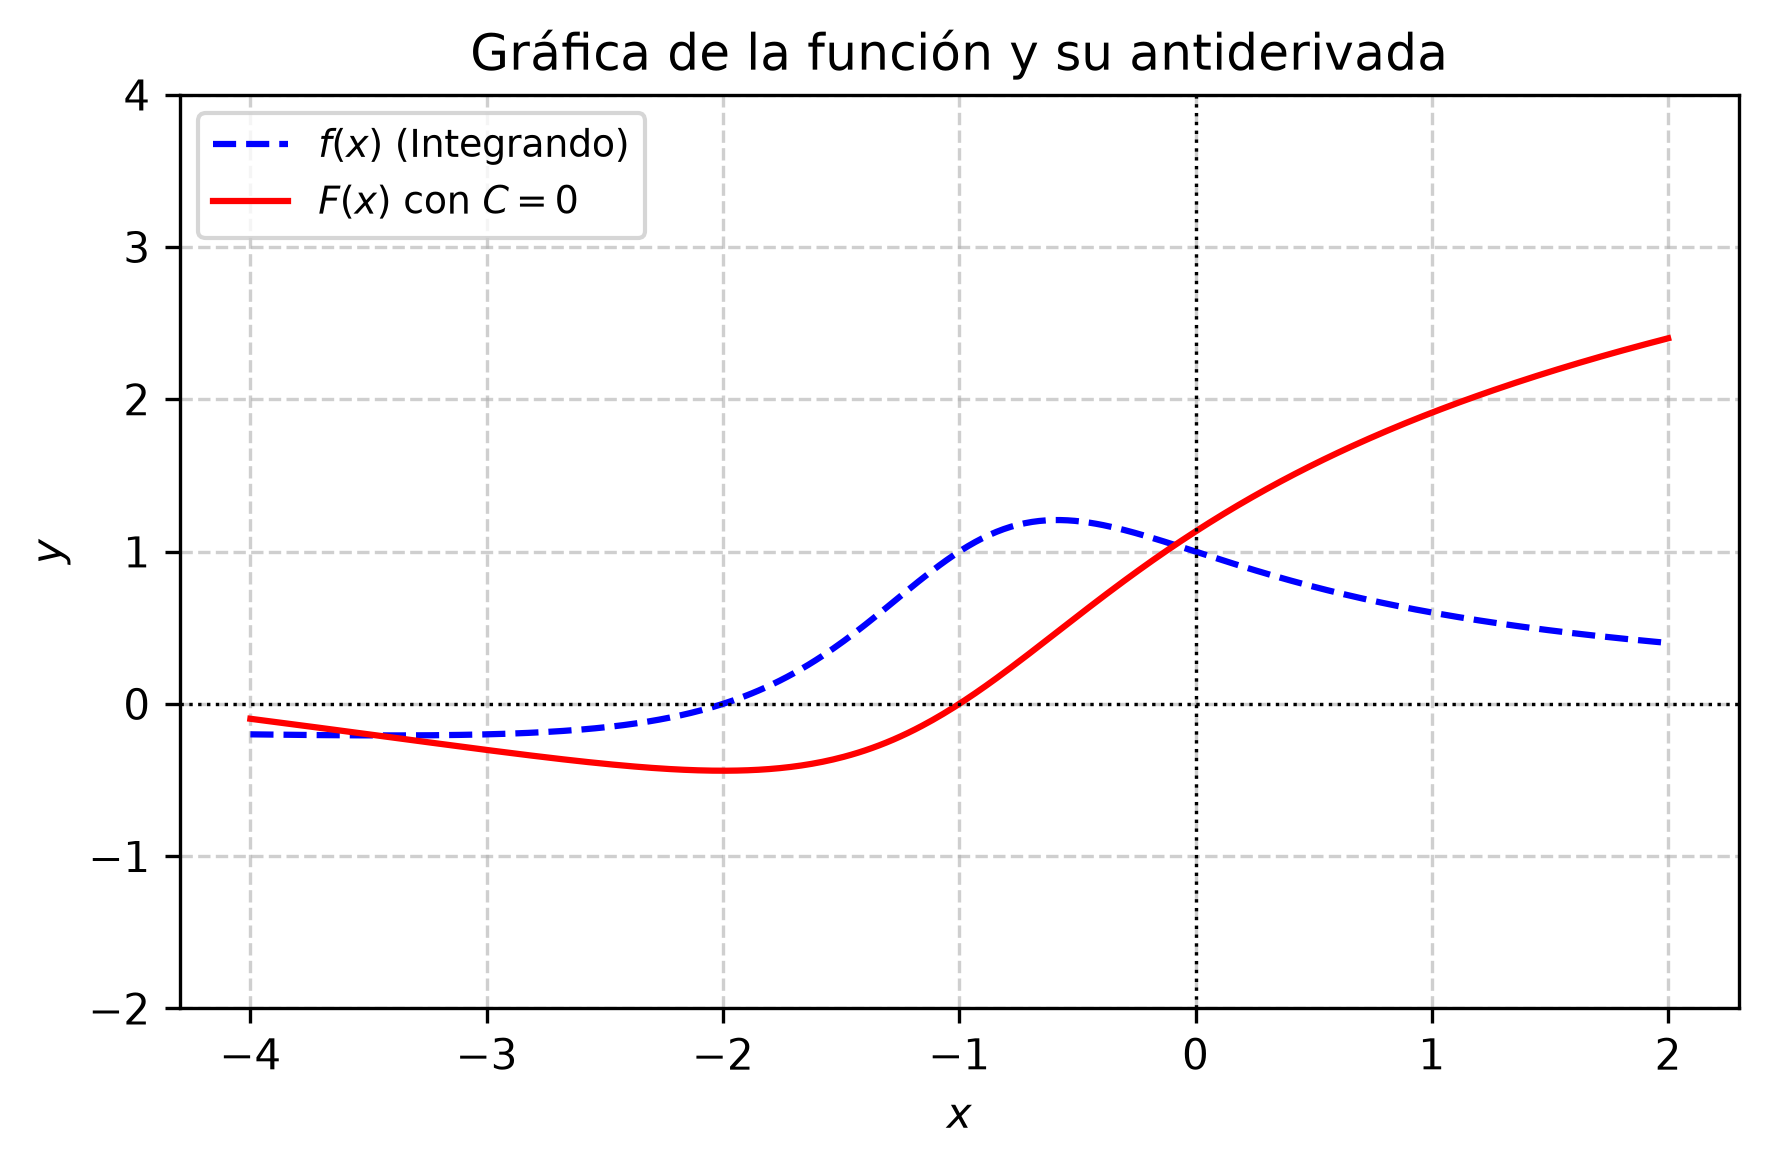
\includegraphics[width=\columnwidth]{semana_03/graficas/SEM03_P06_grafica.png}
	\caption{Representación gráfica de $f(x)$ y su antiderivada $F(x)$ evaluada para la constante de integración $C = 0$ (Problema 06).}
	\label{fig:problema06}
\end{figure}
